\subsection{Regions of a Tokamak Plasma} \label{sub:RegionsOfPlasma}

\begin{figure}
	\centering
	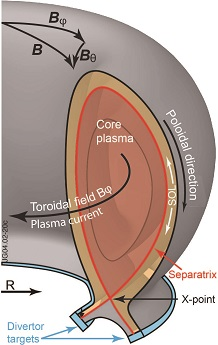
\includegraphics[width=0.5\linewidth]{images/RegionsOfaTokamakPlasma}
	\caption[Features of a Tokamak Plasma\cite{LipschultzBandSharples}]{}
	\label{fig:featuressofatokamakplasma}
\end{figure}

High level features of a tokamak plasma are illustrated in the \prettyref{fig:featuressofatokamakplasma}. These regions include the Core Plasma, the \acf{SOL}, which will sometimes be referred to as the edge region, the Separatrix, which will also be referred to as the \acf{LCFS}, and the X-Point, which is a feature of a divertor design. Also illustrated in this figure is the major radius, R, which is measured from the central axis of the torus. The toroidal direction, $\varphi$, and the poloidal direction are represented. In accordance with these directions, the magnetic field $\vec{B}$ is decomposed into a direction aligned with the toroidal direction, $\vec{B_\varphi}$ and a component that is in the poloidal direction, $\vec{B_\theta}$. Velocity can be decomposed as either parallel to $\vec{B}$, $\left(V_\parallel\right)$, perpendicular to $\vec{B}$, $\left(V_\perp\right)$ or along one of the toroidal directions $\left(V_\varphi \text{ or } V_\varTheta\right)$. The minor axis, r, which is not illustrated here, extends from the plasma magnetic center to the outer wall. For this reason, the radius that works its way into equations is not a fixed value but is given by \cref{eqn:Radius}
%
\begin{equation}
	R\left(r\right) = R_0 + r\cos \theta
	\label{eqn:Radius}
\end{equation}
%
where, $R_0$ is the radial distance from toroidal center to the magnetic center. Because, this analytical approach is one-dimensional $\theta = 0$ and $R\left(r\right)$ is simply $R_0 + r$
